\documentclass[a4paper,11pt]{article}

\usepackage[latin1]{inputenc}
\usepackage[T1]{fontenc}
\usepackage{bbm} %math chars
\usepackage{amsmath}
\usepackage{indentfirst}
\usepackage{fullpage} %minimizes the default margins
\usepackage{url}
\usepackage{graphicx}
\usepackage[center,footnotesize]{caption} %options des legendes des graphes
\usepackage[section]{placeins} %place les figures d'une section avant le debut de la suivante
\usepackage{subfig} %a) b) c)
\usepackage{fancyvrb}

\title{Solution - Week 10}
\date{}
\author{Genomics and bioinformatics}

\begin{document}
\maketitle


\section{General Notes}
\indent To completely understand the exercises and solutions, you need to understand the paper first. The exercise does not cover all the points in the paper, but guides you through important ones. After completing it, you should be able to reproduce all the figures in this paper and others of its kind.


\section{Getting the data}
 The GEO accession code for this paper's dataset is GSE25107. Since all the NCBI databases are linked (they are actually on the same ftp server), all you need is one accession number for one database (in this case GEO).

\begin{enumerate}
\item From which database would you download the raw sequencing files?

The raw sequencing files would be found in the SRA database (accession code: SRP004431)
\item From which database would you get general information about a specific sample?

You can find that in GEO or in BioSample.
\item What is the difference between the datasets in SRA and those in GEO?

The "wig" format you would find in GEO is a processed file, whereas the SRA is a compressed format for storing raw reads. The SRA database contains raw sequencing files as obtained from the sequencing machines. In this case, they are the output of the Illumina Genome Analyzer II and are text files with all the short reads that have been sequenced. On the other hand, the GEO "wig" files are obtained after mapping those reads to the yeast genome and performing normalization to obtain a quantification of reads throughout the yeast genome. See GSE25107\_RAW.tar (custom).
\end{enumerate}

\section{Viewing the data in UCSC}
\begin{enumerate}
\item In figure 1b in the paper, the authors show a proof of principle of their NET-seq protocol by comparing it to RNA-seq. Upload the appropriate tracks to the genome browser and zoom to the RPL30 gene (YGL030W). Do you get the same result?

Since the RPL30 gene is on the + strand, the tracks that you need to upload are: WT\_NC\_plus (for the NET-seq data in the wild-type) and WT\_mRNA\_plus (for the RNA-seq in the wild-type). Notice that there are many reads mapping to the intron in the NET-seq data, but not the RNA-seq data (figure 1)

\begin{figure}[h]
\begin{center}
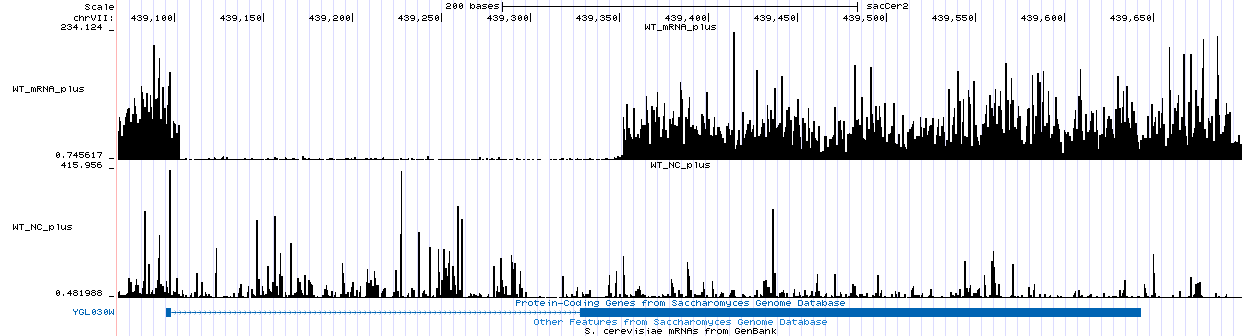
\includegraphics[width=1\textwidth]{solution-figure1-Q3-1.png}
\caption{UCSC view of of the RPL30 gene}
\label{fig:HMM}
\end{center}
\end{figure}

\item The authors talk about CUTs in the paper. What are they?

Cryptic unstable transcripts (CUTs) are a class of short transcripts that are upstream and antisense to an annotated gene. They are degraded quickly, so they will always be undetected by RNA-seq. The biological function of these transcripts, if it exists, is not yet known.

\item Visualize the CUTs in the cluster of genes in figure 3a (make sure you upload the appropriate tracks). What do you notice when you compare \textit{RCO1$\Delta$} to the wild-type?

For this exercise, you will need to upload the following tracks:
\begin{itemize}
\item WT\_NC\_plus
\item WT\_NC\_minus
\item RCO1D\_plus
\item RCO1D\_minus
\end{itemize}

Then you will need to navigate to a window where you could see all those genes like: chrVII:662,257-675,621 (figure 2). Notice the CUT sites in the "minus" tracks. Also notice that the RCO1D deletion mutant has a higher CUT expression (up to 533.394 reads per 10\textsuperscript{7})

\begin{figure}[h]
\begin{center}
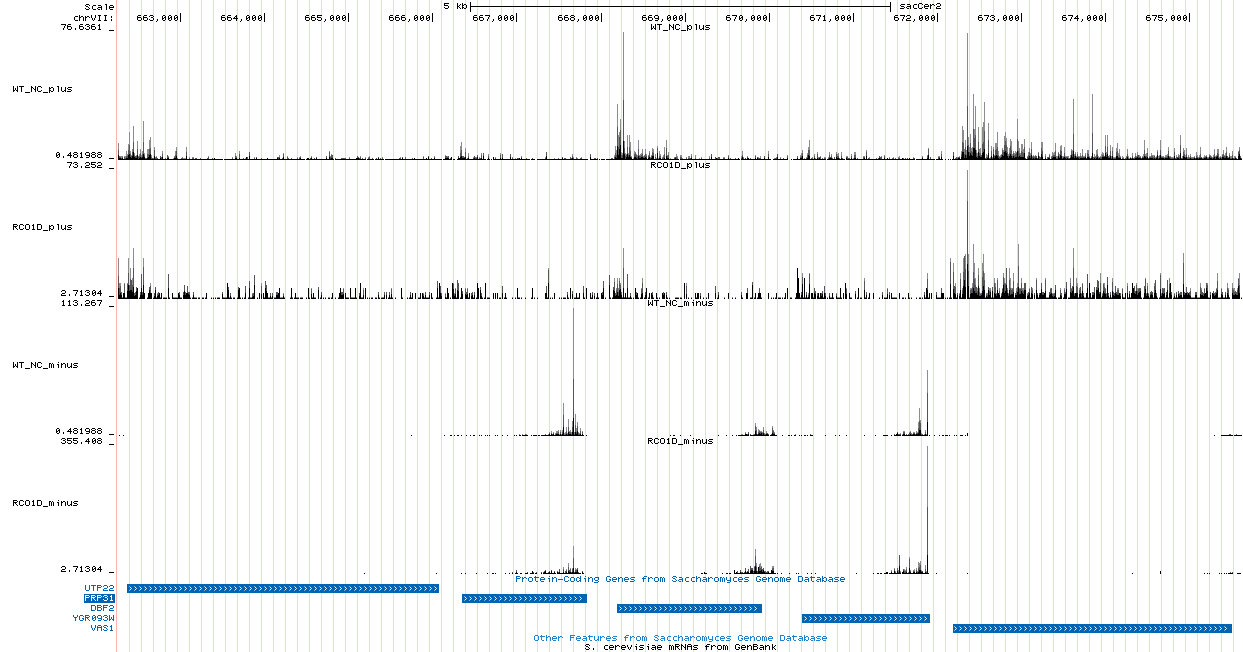
\includegraphics[width=1\textwidth]{solution-figure2-Q3-2.png}
\caption{UCSC view of of the genes in the paper's figure 3a}
\label{fig:HMM}
\end{center}
\end{figure}

\item For the next exercise, you will need to extract gene annotation information (like strand and transcription start) for all the genes on chromosome VII. This is easy to do in UCSC. Go to Tools>Table Browser. Under group, select Genes and Gene Prediction Tracks, then select SGD Genes in the track drop down list. Define the position as "chrVII" and then click on get output. Observe the resulting table, for this will be useful for the next exercise.

\begin{figure}[h]
\begin{center}
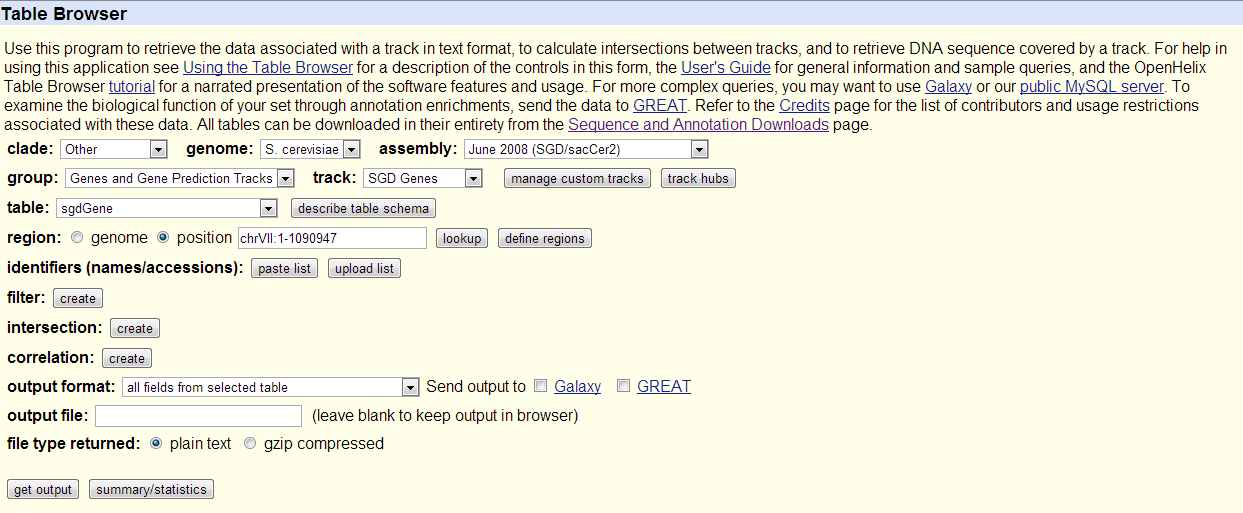
\includegraphics[width=1\textwidth]{solution-figure3-Q3-3.png}
\caption{UCSC table browser snapshot}
\label{fig:HMM}
\end{center}
\end{figure}

\end{enumerate}

\section{Reproducing figures in R or Python}
\begin{enumerate}
\item Try to reproduce figure 1b in R or Python. You will need to load the appropriate ".wig" files and to extract the region corresponding to the RPL30 gene. You can find a text file on moodle named \texttt{chrVII\_UCSC.txt}, which contains annotation information of all genes on chromosome VII.

You can find two solutions for this exercise in R. One is more complicated than the other.

\item Explain the significance of figure 3b and try to reproduce it.

In figure 2d, the authors show that there is a strong correlation between antisense transcription and histone H4 acetylation. So, to test if there is a causal role of this acetylation, they perform NET-seq on a yeast strain that has no RCO1 (a required subunit of the Rpd3S histone 4 deacetylation complex). And indeed, they observe a higher antisense/sense ratio in the mutant when compared to the control (figure 3b).

The R solution is in the same file as that of the previous exercise.
\end{enumerate}


\end{document}











